\documentclass[a4paper,11pt]{article}
\usepackage[portuguese]{babel}
\usepackage{graphicx}
\usepackage{amsmath}
\usepackage{minted}
\usepackage{enumitem}


\title{Estruturas de Dados\\ Resolução de exercícios de testes}
\author{Eduardo Freitas Fernandes}
\date{2025}

\setminted{
	frame=single,
	tabsize=4,
	breaklines=true
}

\begin{document}
	
\maketitle
	
	
\noindent \textbf{Exercício 1}

\begin{minted}{c}
int hash(char matricula[6]) {
	unsigned int hash = 0;
	unsigned int base = 31; // número primo
	
	while (*matricula != '\0') {
		hash = hash * base + (unsigned int) (*matricula);
		matricula++;
	}
	
	return hash;
}
\end{minted}

\begin{minted}{c}
int insert(Tabela t, char matricula[6]) {
	int index = hash(matricula) % SIZE;
	struct no ** temp = &(t[index]);
	
	while (*temp != NULL && strcmp((*temp)->matricula, matricula)) {
		temp = &((*temp)->next);
	}
	
	if (*temp == NULL) {
		*temp = malloc(sizeof(struct no));
		strcpy((*temp)->matricula, matricula);
		(*temp)->next = NULL;
	}
	
	return index;
}
\end{minted}

	
\noindent \textbf{Exercício 2}

\begin{minted}{c}
#define LEFT (-1)
#define BALANCED 0
#define RIGHT 1

Arvore rr(Arvore arv) {
	Arvore left = arv->esq;
	int root_status = arv->bal;
	int left_status = left->bal;
	
	arv->esq = left->dir;
	left->dir = arv;
	
	if (root_status == RIGHT && left_status <= BALANCED)
		arv->bal = BALANCED;
	else
		arv->bal = LEFT;
	
	return left;
}
\end{minted}

	
\noindent \textbf{Exercício 3}\\
\[
	T(N) =
	\begin{cases}
		0 & N \leq 0 \\
		2 \times T_{altura}(N/2) + 2 \times T(N/2) & N > 0
	\end{cases}
\]
\[
	=
	\begin{cases}
		0 & N \leq 0 \\
		N + 2 \times T(N/2) & N > 0
	\end{cases}
	= \sum_{i=1}^{1+\log_2(N)} N = \Theta(N \times \log_2(N))
\]
	
\noindent \textbf{Exercício 4}

\begin{minted}{c}
void sinonimos(Dic d, char *pal) {
	int index = hash(pal) % TAM;
	struct p *temp = d[index];
	while (temp != NULL && strcmp(temp->pal, pal))
		temp = temp->next;
	if (temp != NULL) {
		struct s *aux = temp->sins;
		while (aux) {
			printf("'%s' == '%s'\n", pal, aux->sin);
			aux = aux->next;
		}
	}
}
\end{minted}

\noindent \textbf{Exercício 5}

\begin{minted}{c}
Tree heapToTreeRec(Heap h, int i, int size) {
	if (i >= size)
		return NULL;
	
	Tree root = malloc(sizeof(struct nodo));
	root->val = h[i];
	root->esq = heapToTreeRec(h, 2 * i + 1, size);
	root->dir = heapToTreeRec(h, 2 * i + 2, size);
	
	return root;
}
	
Tree heapToTree(Heap h, int size) {
	return heapToTreeRec(h, 0, size);
}
\end{minted}

\noindent \textbf{Exercício 6}

\begin{figure}[H]
	\centering
	\begin{minipage}{0.49\textwidth}
		\centering
		\fbox{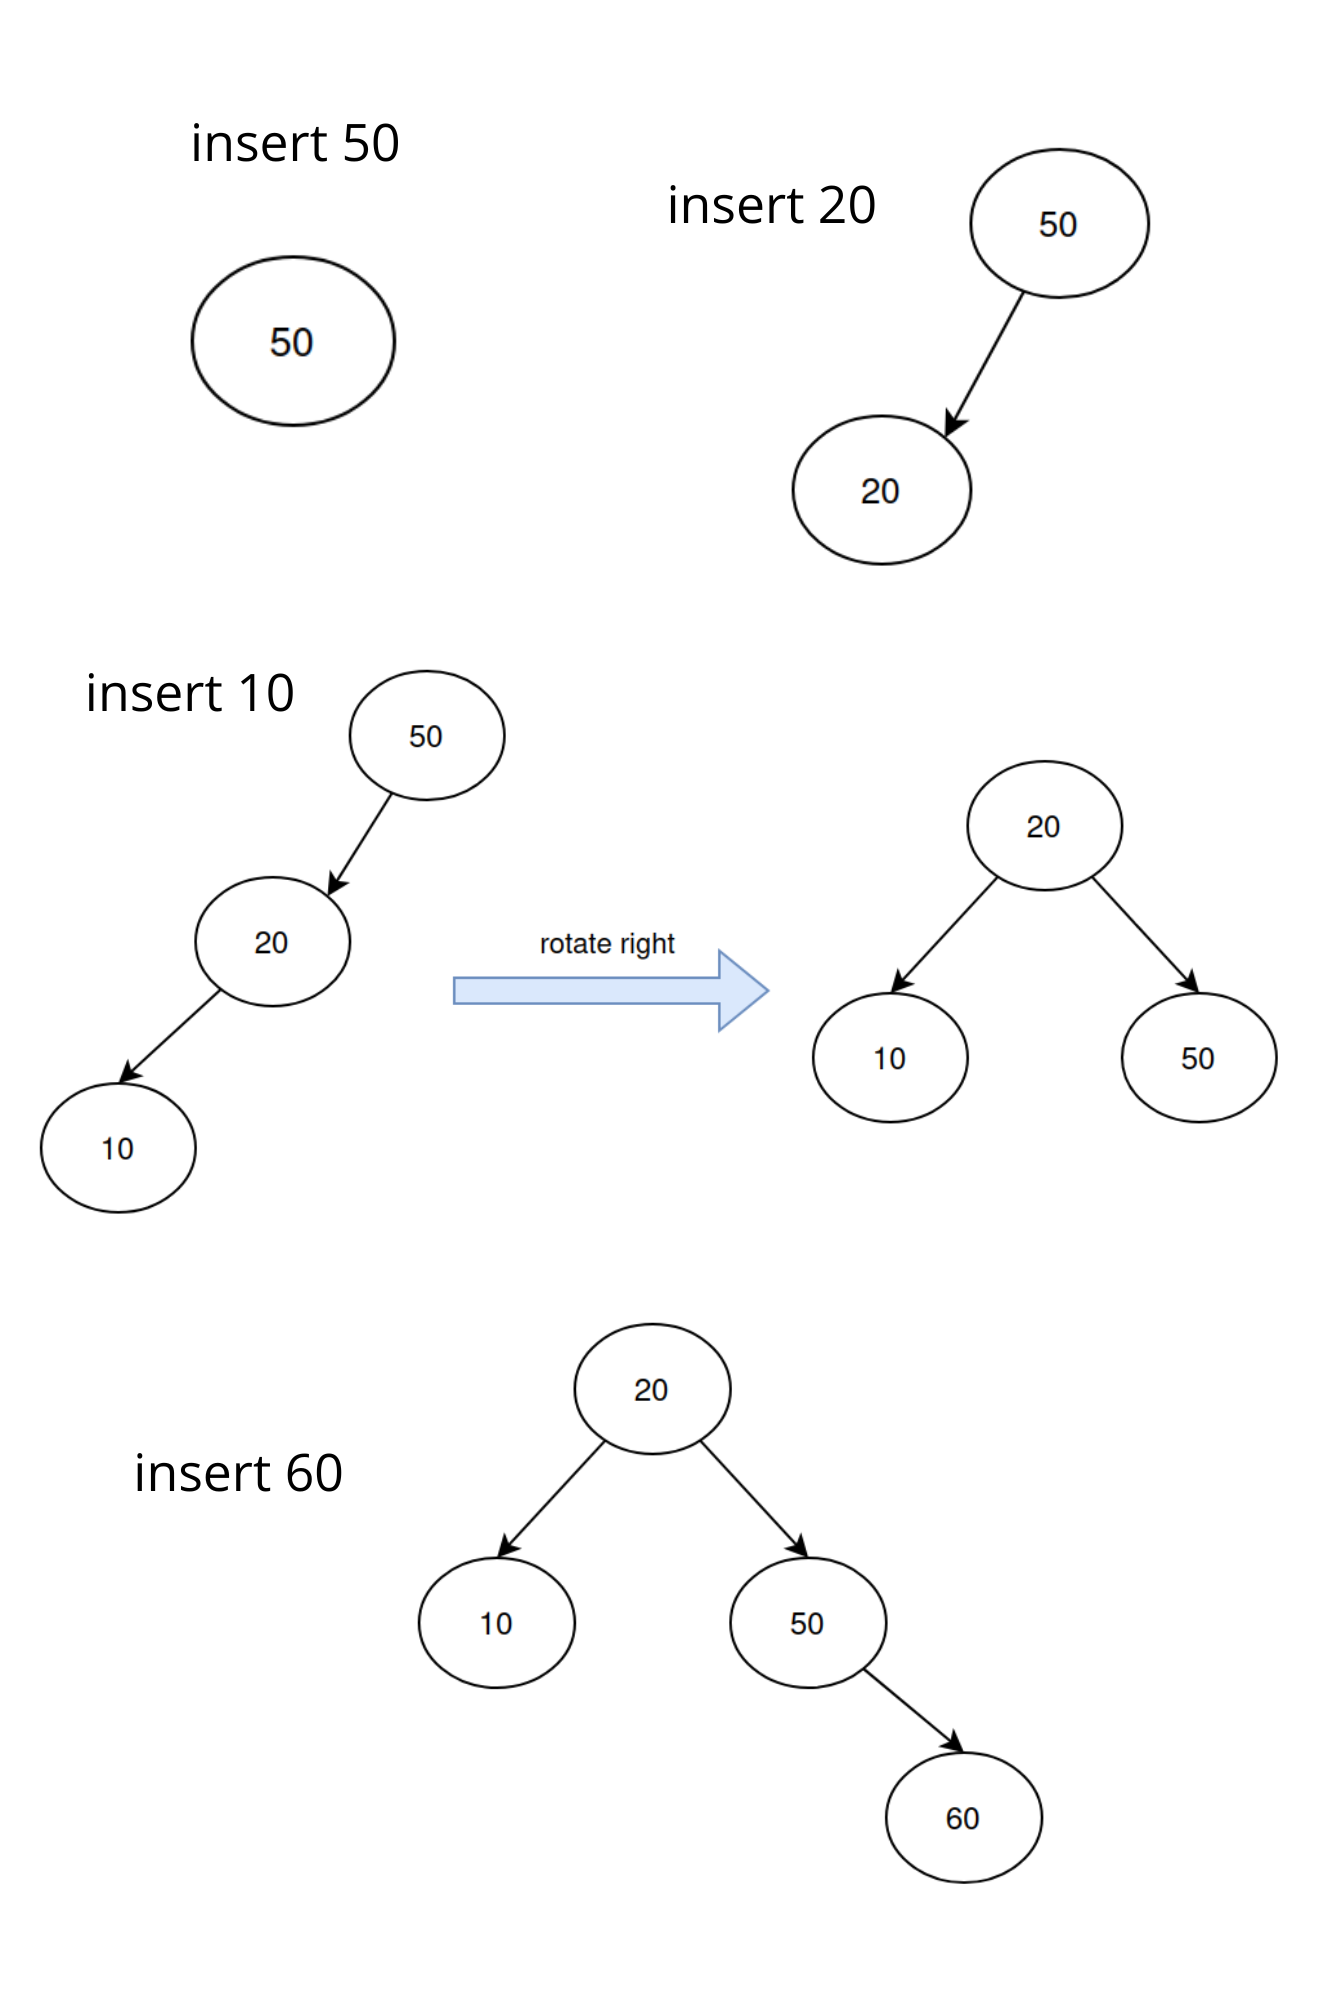
\includegraphics[width=\textwidth]{imgs/6-1.png}}
		\caption{Inserir 50, 20, 10, 60}
	\end{minipage}
	\hfill
	\begin{minipage}{0.49\textwidth}
		\centering
		\fbox{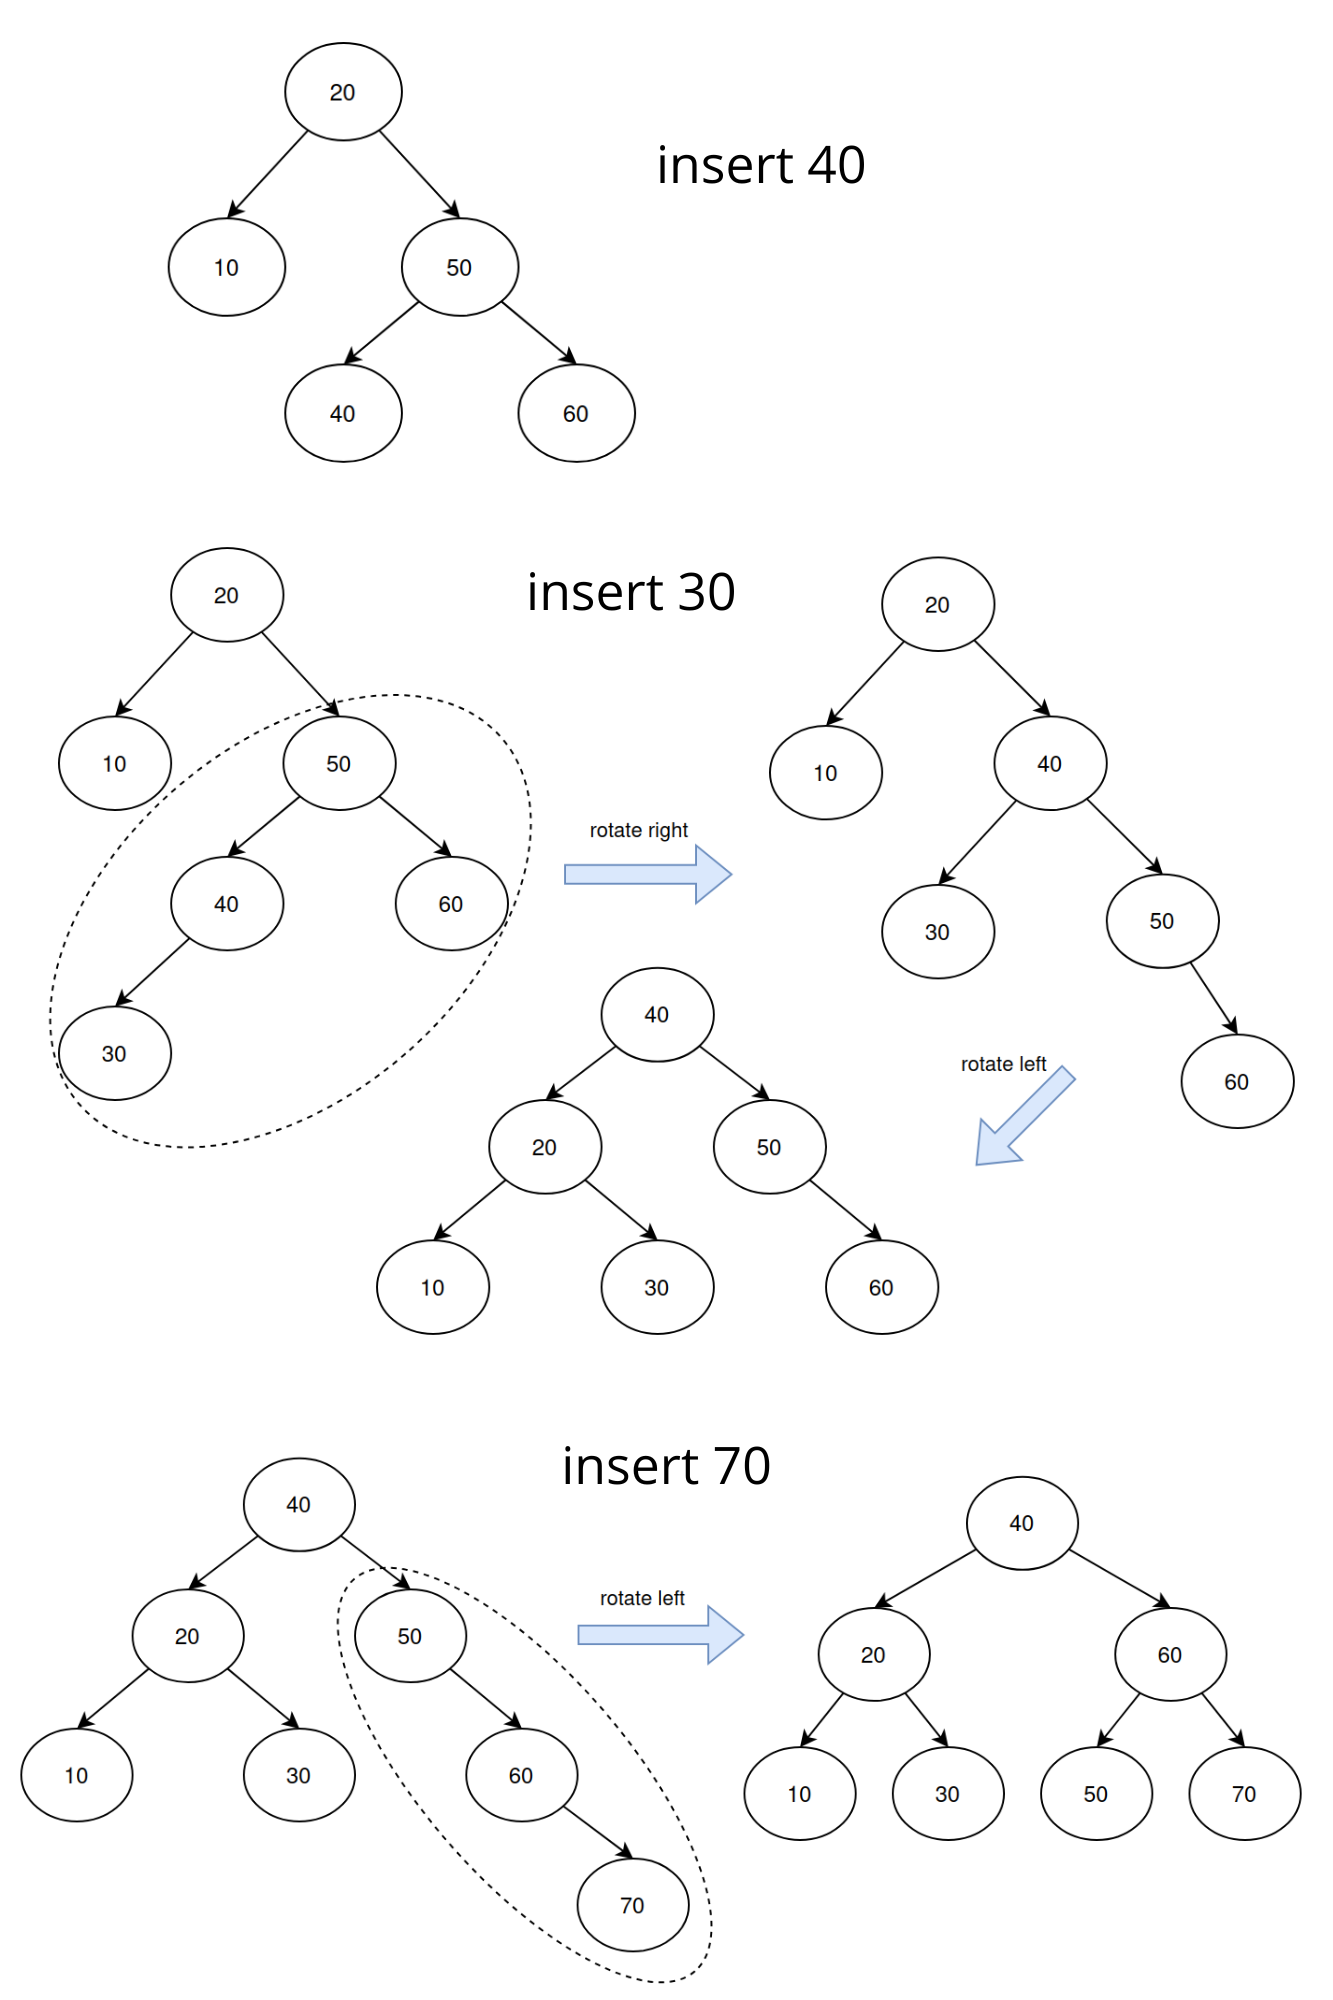
\includegraphics[width=\textwidth]{imgs/6-2.png}}
		\caption{Inserir 40, 30, 70}
	\end{minipage}
\end{figure}

\newpage

\noindent \textbf{Exercício 7}
	
\begin{minted}{c}
Node buildBST(int arr[], int n) {
	if (n <= 0) return NULL;
	
	int middle = n / 2;
	Node root = malloc(sizeof(struct node));
	root->info = arr[middle];
	root->esq = buildBST(arr, middle);
	root->dir = buildBST(arr + middle, n - middle);
	
	return root;
}
\end{minted}

\noindent \textbf{Exercício 8}

\begin{minted}{c}
#define SIZE 1001
typedef struct count {
	char store[SIZE];
	int total;
} Count;

void init_count(Count *c) {
	c->total = 0;
	for (int i = 0; i < SIZE; i++)
		c->store[i] = 0;
}

void insert(Count *c, int x) {
	c->total += c->store[x] == 0 ? 1 : 0;
	c->store[x] = 1;
}

int check(Count *c, int x) { return c->store[x]; }

void show(Count *c) {
	int count = 0, i;
	for (i = 0; i < SIZE && count < c->total; i++) {
		if (c->store[i] != 0)
			printf("%d ", i);
		count += c->store[i];
	}
}
\end{minted}

\noindent \textbf{Exercício 9}

\begin{minted}{c}
#define PARENT(i) ((i - 1) / 2)
#define LEFT(i) (2 * i + 1)
#define RIGHT(i) (2 * i + 2)

void swap(MinHeap h, int i, int j) {
	int temp = h->heap[i];
	h->heap[i] = h->heap[j];
	h->heap[j] = temp;
}

void bubbleUp(MinHeap h, int i) {
	int parent = PARENT(i);
	while (i > 0 && h->heap[parent] > h->heap[i]) {
		swap(h, i, parent);
		i = parent;
		parent = PARENT(parent);
	}
}

void muda (MinHeap h, int pos, int valor) {
	h->heap[pos] = valor;
	bubbleUp(h, pos);
}
\end{minted}

\noindent \textbf{Exercício 10}

\begin{minted}{c}
int procura (ABPInt a, int l, int u) {
	while (a != NULL) {
		if (a->valor < u && a->valor > l)
			return 1;
		
		if (a->valor >= u)
			a = a->esq;
		else if (a->valor <= l)
			a = a->dir;
	}
	
	return 0;
}
\end{minted}

\newpage

\noindent \textbf{Exercício 11}\\

\noindent Análise de complexidade da função \texttt{procura()}:
\begin{itemize}
	\item \textbf{Melhor Caso}: a raiz da árvore está entre \texttt{l} e \texttt{u}.
	\item \textbf{Pior Caso}: os valores guardados na árvore não estão presentes no intervalo definido por \texttt{l} e \texttt{u}, ou estão no último nível da árvore.
\end{itemize}
\[
	T(N) = \sum_{i=1}^{1+\log_2(N)} 1 = 1 + \log_2(N) = \Theta(\log_2(N))
\]

\noindent \textbf{Exercício 12}

\begin{minted}{c}
int biggest(MinHeap *h) {
	// as folhas da heap são os maiores elementos
	// logo basta percorrer apenas esses elementos
	int stop = h->tamanho / 2;
	int max = h->heap[h->tamanho - 1];
	
	for (int i = h->tamanho - 2; i >= 0 && i >= stop; i--)
		if (h->heap[i] > max)
			max = h->heap[i];
	
	return max;
}
\end{minted}

\noindent \textbf{Exercício 13}

\begin{minted}{c}
int rdir(AVL *tptr) {
	if (*tptr == NULL || (*tptr)->esq == NULL)
		return -1;
	
	AVL left = (*tptr)->esq;
	(*tptr)->esq = left->dir;
	*tptr = left;
	
	return 0;
}
\end{minted}

\newpage

\noindent \textbf{Exercício 14}

\begin{figure}[h]
	\centering
	\fbox{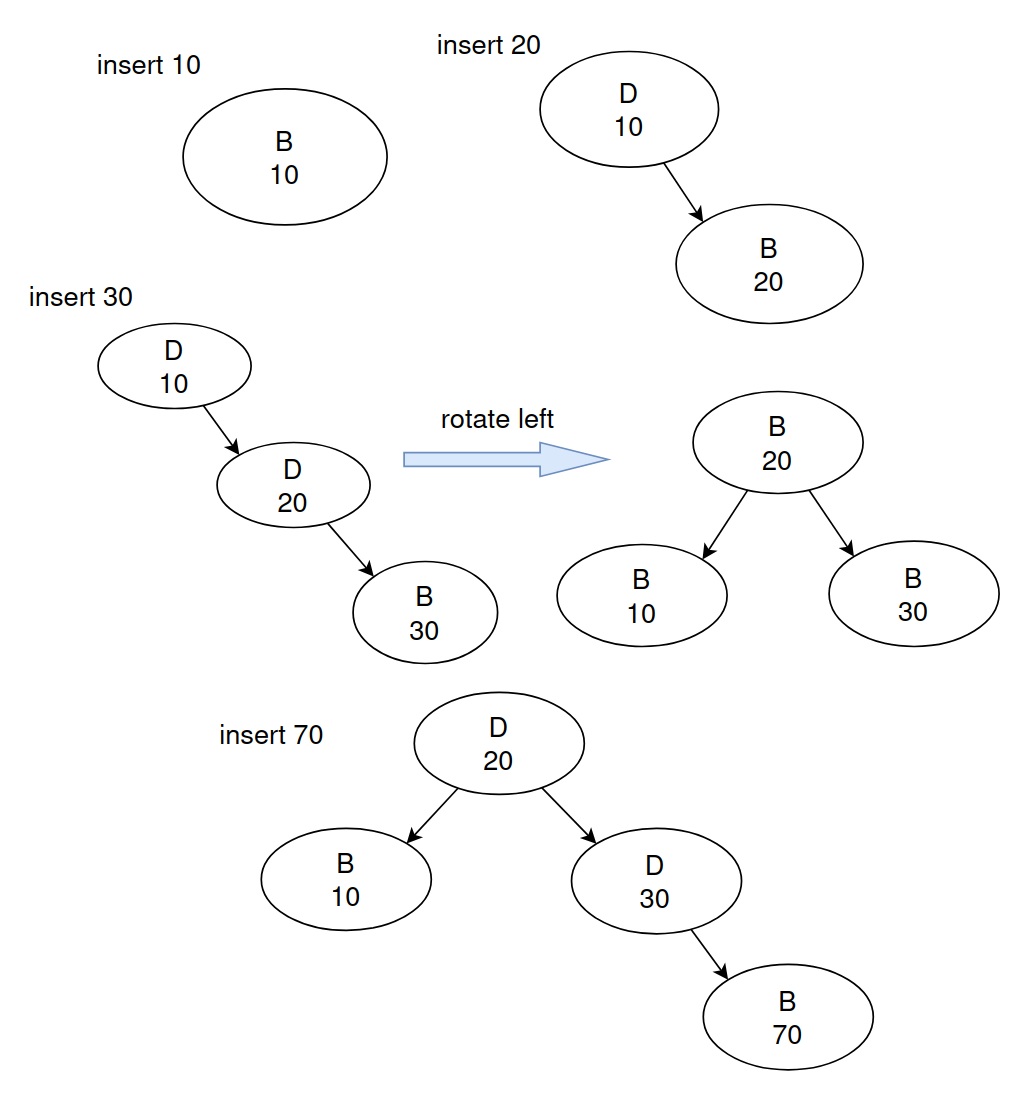
\includegraphics[width=0.7\textwidth]{imgs/14-1.png}}
	\caption{Inserir 10, 20, 30, 70}
\end{figure}

\begin{figure}[H]
	\centering
	\fbox{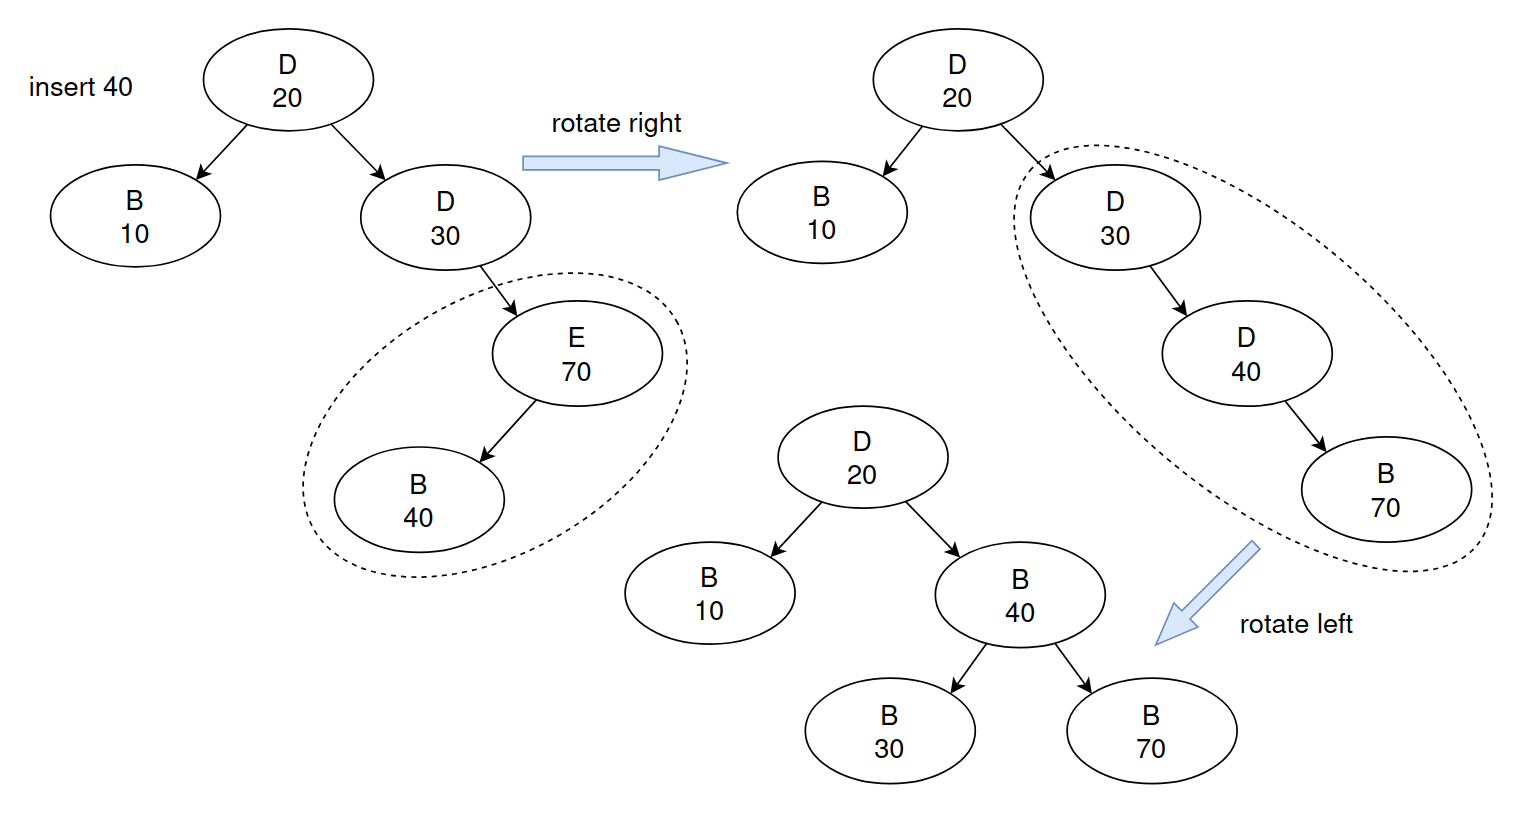
\includegraphics[width=0.9\textwidth]{imgs/14-2.png}}
	\caption{Inserir 40}
\end{figure}

\begin{figure}[H]
	\centering
	\fbox{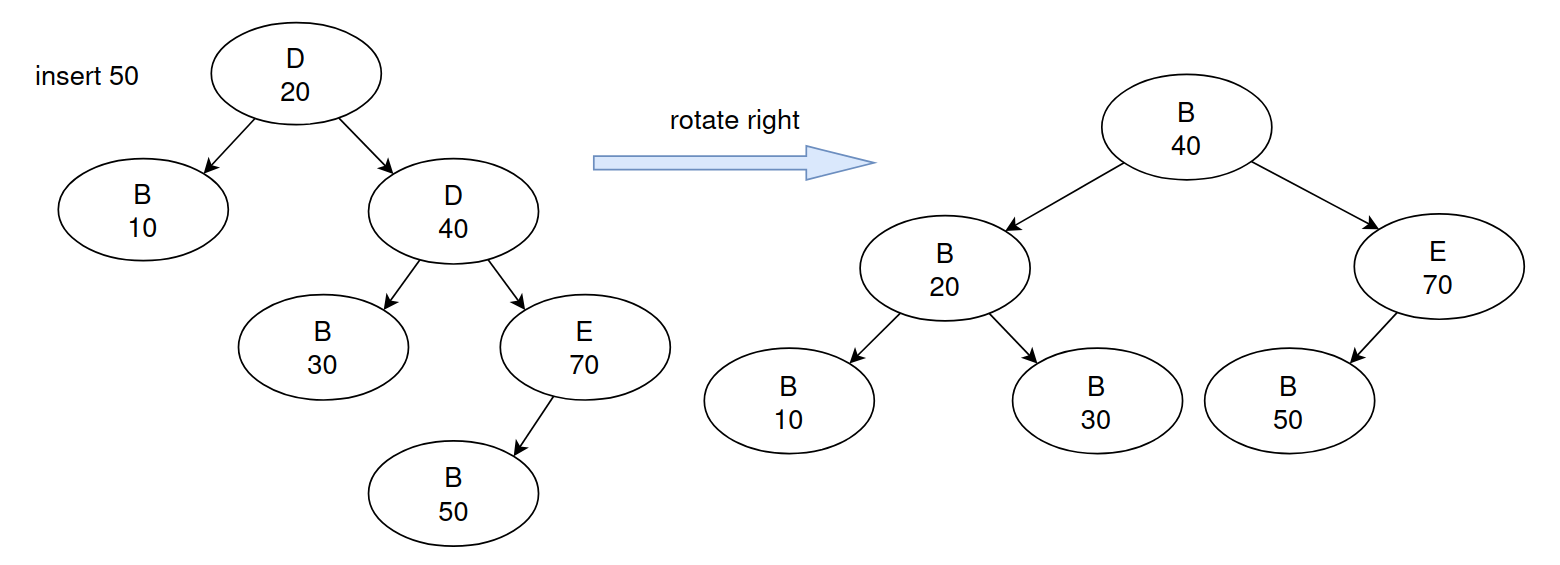
\includegraphics[width=0.8\textwidth]{imgs/14-3.png}}
	\caption{Inserir 50}
\end{figure}


\noindent \textbf{Exercício 15}\\

\noindent Tabelas de Hash:
\begin{enumerate}[label=\alph*)]
	\item quando todas as \texttt{n} inserções colidem na mesma posição, tornando a tabela de hash numa lista ligada, com complexidade de O(N) na pesquisa.
	\item 
	\item
\end{enumerate}

\noindent \textbf{Exercício 16}

\begin{figure}[H]
	\centering
	\fbox{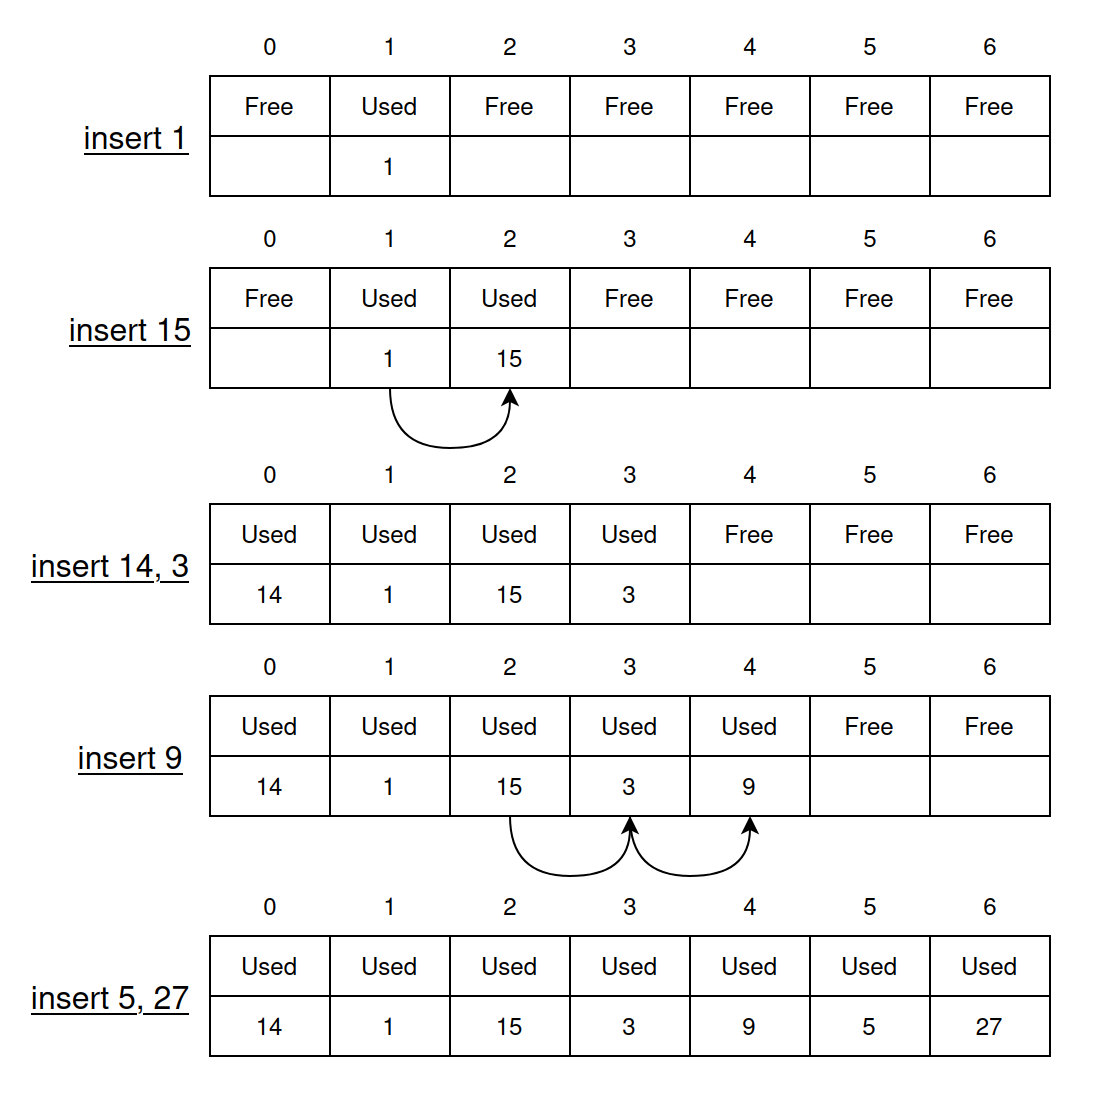
\includegraphics[width=0.8\textwidth]{imgs/16-1.png}}
	\caption{Inserir 1, 15, 14, 3, 9, 5 e 27}
\end{figure}

\begin{figure}[H]
	\centering
	\fbox{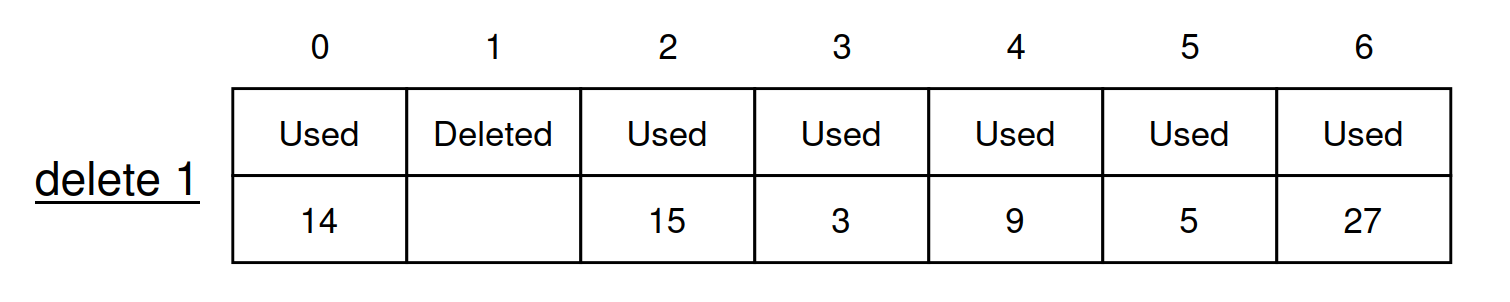
\includegraphics[width=0.8\textwidth]{imgs/16-2.png}}
	\caption{Remover 1}
\end{figure}

\noindent \textbf{Exercício 17}

\begin{figure}[h]
	\centering
	\fbox{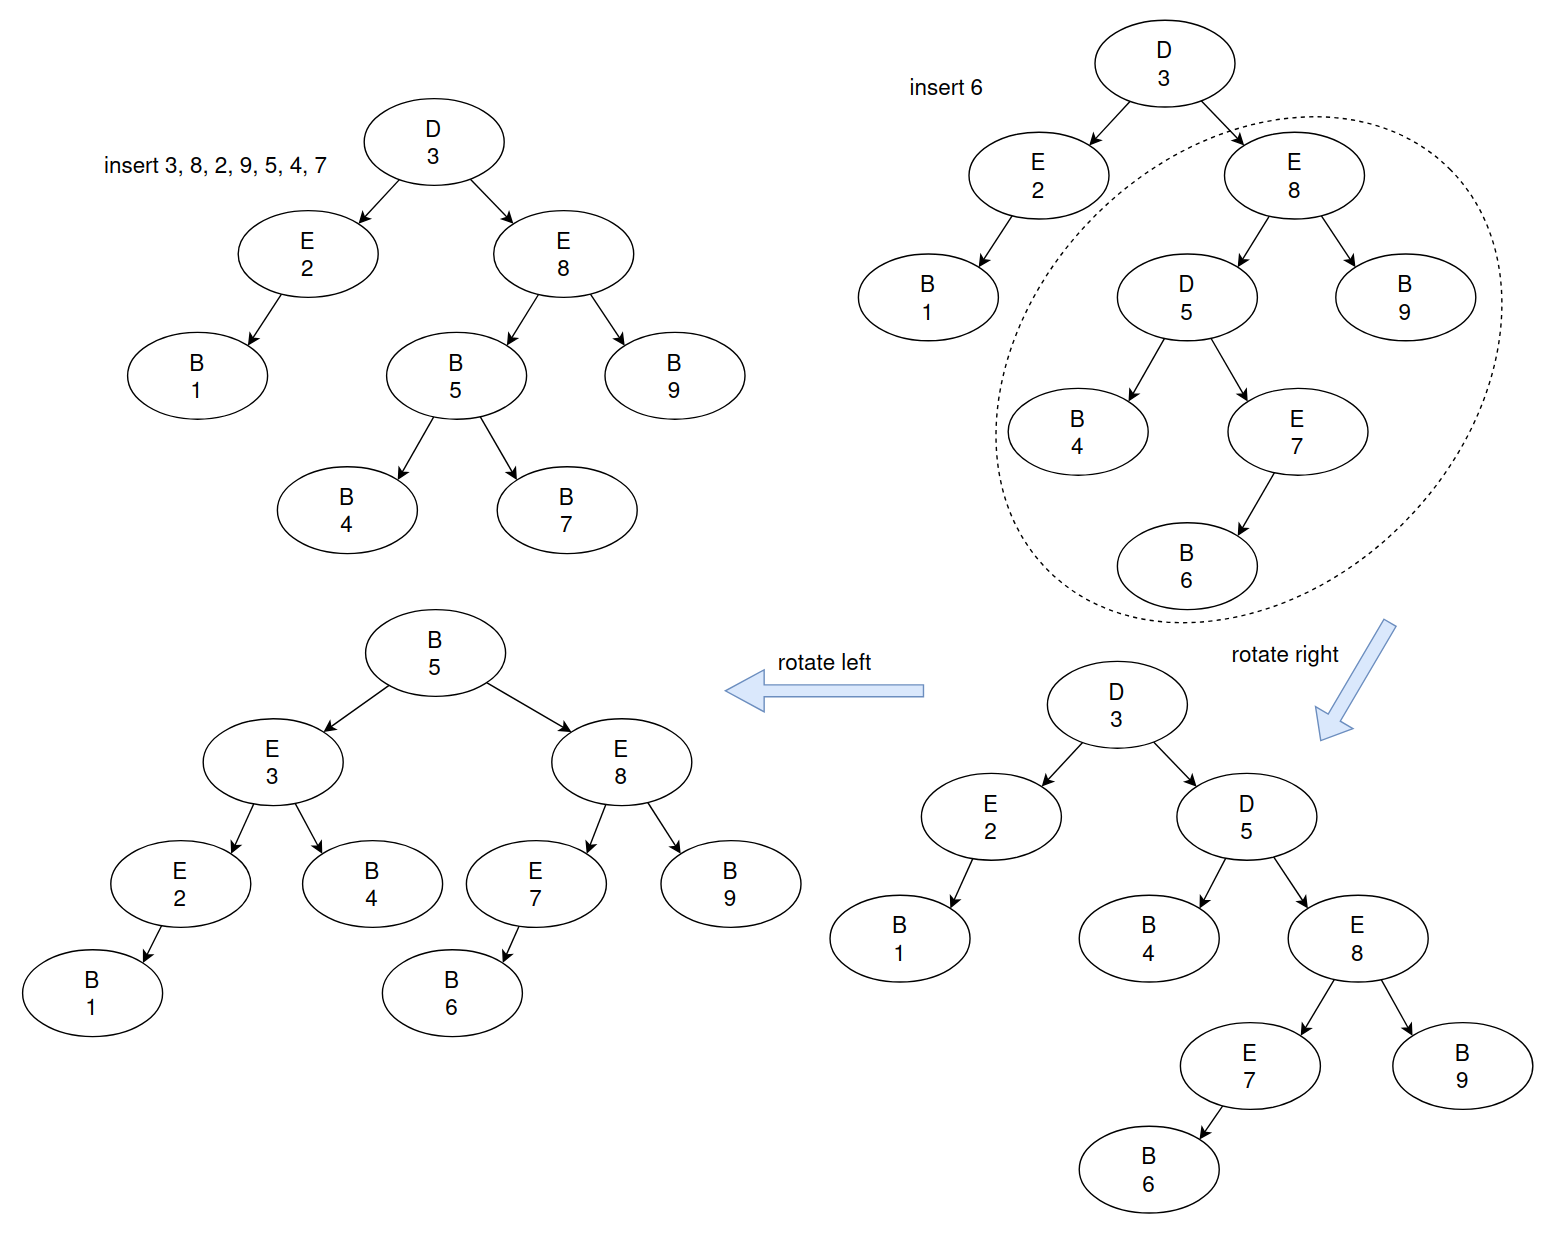
\includegraphics[width=0.9\textwidth]{imgs/17.png}}
	\caption{Árvore AVL}
\end{figure}

\noindent \textbf{Exercício 18}\\

\noindent Tabela de Hash com resolução de colisões por Chaining:

\begin{itemize}
	\item 
	\item 
\end{itemize}

\noindent \textbf{Exercício 19}

\begin{minted}{c}
void swap(int * array, int i, int j) {
	int temp = array[i];
	array[i] = array[j];
	array[j] = temp;
}

int *ordenados (MinHeap h) {
	int *ord = calloc(h->used, sizeof(int));
	
	for (int i = 0; i < h->used; i++) {
		ord[i] = h->values[0];
		swap(h->values, 0, h->used - 1 - i);
		bubbleDown(h); // coloca a raiz no nível correto
	}
	
	free(h->values);
	free(h);
	
	return ord;
}
\end{minted}

\noindent \textbf{Exercício 20}\\

\noindent Nesta tabela, o fator de carga, é o tamanho médio de cada lista, ou seja, o número médio de colisões, logo: \texttt{load = used / size}

\begin{minted}{c}
float loadFactorC (HashTableChain t) {
	int count = 0;
	EntryChain *temp = NULL;
	for (int i = 0; i < t->hashsize; i++) {
		temp = (t->table) + i;
		while(temp != NULL) {
			count++;
			temp = temp->next;
		}
	}
	
	return count / (float) t->hashsize;
}
\end{minted}

\noindent \textbf{Exercício 21}

\begin{minted}{c}
int hash (int size, char key[]) {
	int res = 0;
	for (int i = 0; key[i] != '\0'; i++)
		res += rank[tolower(key[i]) - 'a'];
	
	return res % size;
}
\end{minted}

\noindent \textbf{Exercício 22}



\noindent \textbf{Exercício 23}


\[
	T_{hToAux}(N) =
	\begin{cases}
		0 & N \leq 0 \\
		1 + T_{hToAux}(N/2) & N > 0
	\end{cases}
\]
\[
	= \sum_{i=0}^{1+\log_2(N)} 2^i = 4 \times N - 1 = \Theta(N)
\]

\noindent \textbf{Exercício 24}

\begin{minted}{c}
int hash(char * key);

void doubleTable (HashTableOAddr h) {
	int d_size = 2 * h->size, index = 0;
	EntryOAdd * new = calloc(d_size, sizeof(EntryOAdd));
	// não é necessário inicializar os buckets a FREE
	// calloc() faz isso
	
	for (int i = 0; i < h->size; i++) {
		index = hash(h->table[i].key) % d_size;
		while(new[index].status != STATUS_FREE)
			index = (index + 1) % d_size;
		
		new[index].status = STATUS_USED;
		new[index].info = h->table[i].info;
		new[index].key = h->table[i].key;
	}
	
	h->size = d_size;
	free(h->table);
	h->table = new;
}
\end{minted}

\noindent \textbf{Exercício 25}

\begin{minted}{c}
#define SIZE 1001
typedef struct count {
	int store[SIZE];
	int total;
} Count;

void init_count(Count *c) {
	c->total = 0;
	for (int i = 0; i < SIZE; i++)
		c->store[i] = 0;
}

void insert(Count *c, int x) {
	c->store[x]++;
	c->total++;
}

int check(Count *c, int x) { return c->store[x]; }

void show(Count *c) {
	int count = 0, i, j;
	for (i = 0; i < SIZE && count < c->total; i++) {
		for (j = 0; j < c->store[i]; j++)
			printf("%d ", i);
		count += c->store[i];
	}
}
\end{minted}

\noindent \textbf{Exercício 26}

\begin{minted}{c}
#define PARENT(i) ((i - 1) / 2)
#define LEFT(i) (2 * i + 1)
#define RIGHT(i) (2 * i + 2)

int menor(MinHeap h, int i) {
	if (i >= h->used) return 1;
	
	int left = LEFT(i);
	if (left < h->used && h->values[i] > h->values[left])
		return 0;
	
	int right = RIGHT(i);
	if (right < h->used && h->values[i] > h->values[right])
		return 0;
	
	return menor(h, left) && menor(h, right);
}

int minHeapOk(MinHeap h) {
	return menor(h, 0);
}
\end{minted}

\noindent \textbf{Exercício 27}

\begin{minted}{c}
HashTable newTable(int hashsize) {
	HashTable new = malloc(sizeof(struct hashT));
	new->hashsize = hashsize;
	new->table = malloc(hashsize * sizeof(Entry));
	for (int i = 0; i < hashsize; i++)
		new->table[i] = NULL;
	
	return new;
}
\end{minted}

\noindent \textbf{Exercício 28}



\noindent \textbf{Exercício 29}

\begin{minted}{c}
int altura(AVL a) {
	int height = 0;
	while (a != NULL) {
		a = a->bal == Dir ? a->dir : a->esq;
		height++;
	}
	
	return height;
}
\end{minted}

\noindent \textbf{Exercício 30}

\begin{minted}{c}
AVL rotateLeft(AVL a) {
	AVL right = a->dir;
	int root_height = a->altura;
	int left_diff = root_height - a->esq->altura;
	int right_diff = root_height - right->altura;
	
	if (left_diff <= right_diff) {
		right->altura = root_height + 1;
	} else {
		a->altura--;
		right->altura++;
	}
	
	a->dir = right->esq;
	right->esq = a;
	
	return right;
}
\end{minted}

\noindent \textbf{Exercício 31}

\begin{minted}{c}
void remApagados(THash h) {
	int i, index;
	struct celula * temp = malloc(sizeof(struct celula) * h->tamanho);
	for (i = 0; i < h->tamanho; i++)
		h->Tabela[i].estado = Livre;
	
	for (i = 0; i < h->tamanho; i++) {
		if (h->Tabela[i].estado == Ocupado) {
			index = hash(h->Tabela[i].k, h->tamanho);
			while (temp[index].estado == Ocupado)
				index = (index + 1) % h->tamanho;
			
			temp[index].estado = Ocupado;
			temp[index].info = h->Tabela[i].info;
			temp[index].k = h->Tabela[i].k;
		}
	}
	
	h->apagados = 0;
	free(h->Tabela);
	h->Tabela = temp;
}
\end{minted}

\noindent \textbf{Exercício 32}



\noindent \textbf{Exercício 33}\\

\noindent O valor de balanço presente em cada nodo da árvore indica o lado da árvore que tem maior altura, logo seguindo o caminho indicado pelo balanço dos nodos, chegamos ao nível mais profundo da árvore, obtendo a sua altura. A complexidade é logarítmica, pois a função percorre todos os níveis da árvore, apenas uma vez.

\begin{minted}{c}
int altura(AVL arv) {
	int height = 0;
	
	while (arv != NULL) {
		arv = arv->balanco == Dir ? arv->dir : arv->esq;
		height++;
	}
	
	return height;
}
\end{minted}

\noindent \textbf{Exercício 34}
\[
	T_{extractMin}(N) = \Theta(\log_2(N)) \quad T_{insertTree}(N) = \Theta(\log_2(N))
\]
\[
	T_{heap2AVL}(N) = 
\]

\noindent \textbf{Exercício 35}

\begin{minted}{c}
int allCopies(Dictionary dic, char key[11]) {
	if (dic == NULL) return 0;
	
	int count = 0;
	int comp = strcmp(dic->key, key);
	
	if (comp == 0) {
		count++;
		count += allCopies(dic->left, key);
		count += allCopies(dic->right, key);
	} else if (comp < 0)
		count += allCopies(dic->right, key);
	else
		count += allCopies(dic->left, key);
	
	return count;
}

\end{minted}

\noindent \textbf{Exercício 36}

\begin{minted}{c}
int heapOKRec(BTree arv, int value) {
	if (arv == NULL) return 1;
	if (value > arv->value) return 0;
	return heapOKRec(arv->left, arv->value) &&
		   heapOKRec(arv->right, arv->value);
}

int heapOK(BTree a) {
	return a == NULL || heapOKRec(a, a->value);
}
\end{minted}

\noindent \textbf{Exercício 37}

\begin{minted}{c}
#define PARENT(i) (i - 1) / 2
#define LEFT(i) 2 * i + 1
#define RIGHT(i) 2 * i + 2

void swap(int * array, int i, int j) {
	int temp = array[i];
	array[i] = array[j];
	array[j] = temp;
}

void bubbleUp(int * array, int i) {
	int parent = PARENT(i);
	while (i > 0 && array[parent] > array[i]) {
		swap(array, i, parent);
		i = parent;
		parent = PARENT(parent);
	}
}

void insertHeap(Heap *h, int x) {
	if (h->used == h->size) {
		h->size *= 2;
		h->heap = realloc(h->heap, h->size * sizeof(int));
	}
	
	h->heap[h->used] = x;
	bubbleUp(h->heap, h->used++);
}

\end{minted}

\noindent \textbf{Exercício 38}~
\[
	T_{heapify}(N) = 
\]

\noindent \textbf{Exercício 39}
\[
T_{deepest}(N) = 
\begin{cases}
	0 & N \leq 0 \\
	1 + 2 \times T(N/2) & N > 0
\end{cases}
= \sum_{i=0}^{1+\log_2(N)} 2^i = 4 \times N - 1 = \Theta(N)
\]

\begin{minted}{c}
int deepest(AVLTree *a) {
	if (*a == NULL) return 0; 
	int height = 1;
	while (*a != NULL && ((*a)->left != NULL || 
						  (*a)->right != NULL)) {
		a = (*a)->bal == Right ?
					&((*a)->right) : &((*a)->left);
		height++;
	}
		
	return height;
}
\end{minted}
\[
T_{deepest}(N) = \Theta(\log_2(N))
\]

\noindent \textbf{Exercício 40}

\begin{minted}{c}
int fromChain(HashChain h1, HashOpen h2) {
	// estou a assumir que h2 já está inicializada com Livre
	int i, index;
	struct lista * temp = NULL;
	for (i = 0; i < HSIZE; i++) {
		temp = h1[i];
		index = i;
		while (temp != NULL) {
			while (h2[index].estado == 1)
			index = (index + 1) % HSIZE;
			
			h2[index].estado = 1;
			h2[index].valor = temp->valor;
			
			temp = temp->prox;
		}
	}
	return 0;
}
\end{minted}

\begin{minted}{c}
#define CHAIN_SIZE ...
#define OPEN_SIZE ...
int fromChain(HashChain h1, HashOpen h2) {
	// estou a assumir que h2 já está inicializada com Livre
	int i, index;
	struct lista * temp = NULL;
	for (i = 0; i < CHAIN_SIZE; i++) {
		temp = h1[i];
		while (temp != NULL) {
			index = hash(temp->valor, OPEN_SIZE);
			while (h2[index].estado == 1)
				index = (index + 1) % OPEN_SIZE;
			
			h2[index].estado = 1;
			h2[index].valor = temp->valor;
			
			temp = temp->prox;
		}
	}
	return 0;
}
\end{minted}

\noindent \textbf{Exercício 41}


\noindent \textbf{Exercício 42}

\begin{minted}{c}
AVL maisProfundo(AVL a) {
	while (a != NULL && (a->left != NULL || 
						 a->right != NULL))
		a = a->bal == RIGHT ? a->right : a->left;
	
	return a;
}
\end{minted}

\noindent \textbf{Exercício 43}


\noindent \textbf{Exercício 44}

\begin{minted}{c}
AVL fromListRec(LInt *l, int n, int *height) {
	if (n == 0) {
		*height = 0;
		return NULL;
	}
	
	int hL, hR;
	int middle = n / 2;
	AVL left = fromListRec(l, middle, &hL);
	
	AVL root = malloc(sizeof(struct avl));
	root->value = (*l)->value;
	root->left = left;
	
	*l = (*l)->next;
	
	AVL right = fromListRec(l, n - middle - 1, &hR);
	root->right = right;
	
	root->bal = hR - hL;
	*height = (hL > hR ? hL : hR) + 1;
	
	return root;
}

AVL fromList (LInt l, int n) {
	int h;
	return fromListRec(&l, n, &h);
}
\end{minted}

\noindent \textbf{Exercício 45}



\noindent \textbf{Exercício 46}

\begin{minted}{c}
void shrinkTHash(THash h) {
	int small_size = h->tamanho * 2;
	small_size /= 3;
	
	struct entry * temp = calloc(small_size, 
								 sizeof(struct entry));
	int index, i;
	for (i = 0; i < small_size; i++)
		temp[i].status = LIVRE;
	
	for (i = 0; i < h->tamanho; i++) {
		if (h->tabela[i].status == OCUPADO) {
			index = hash(h->tabela[i].value, small_size);
			while (temp[index].status == OCUPADO)
				index = (index + 1) % small_size;
			
			temp[index].status = OCUPADO;
			temp[index].value = h->tabela[i].value;
		}
	}
	
	free(h->tabela);
	h->tabela = temp;
	h->tamanho = small_size;
}

void removeTHash(THash h, int key) {
	int index = hash(key, h->tamanho);
	int count = 0;
	
	while (h->tabela[index].status != LIVRE && 
		   count < h->tamanho) {
		if (h->tabela[index].status == OCUPADO &&
			h->tabela[index].value == key) {
			h->tabela[index].status = APAGADO;
			h->ocupados--;
			break;
		}
		index = (index + 1) % h->tamanho;
		count++;
	}
	
	if ((h->ocupados / (float) h->tamanho) < 0.33)
		shrinkTHash(h);
}
\end{minted}

\noindent \textbf{Exercício 47}

\begin{minted}{c}
AVL rotateRight (AVL a) {
	AVL left = a->esq;
	
	a->esq = left->dir;
	left->dir = a;
	
	return left;
}
\end{minted}
\[
	T_{spine}(N) =
	\begin{cases}
		0 & N \leq 0 \\
		1 + T(N - 1) & N > 0
	\end{cases}
	\quad = \quad \sum_{i=1}^{N} 1 = \Theta(N)
\]
Como a árvore já está em espinha, todos os nodos terão \texttt{a->esq == NULL}, logo o ciclo nunca será executado. Nesta análise estou a contar o número de vezes que a condição do ciclo é avaliada, que corresponde a uma vez por chamada recursiva.


\end{document}
